\documentclass{article}
\usepackage[utf8]{inputenc}
\usepackage[left=0.7in,right=0.7in,top=1in,bottom=0.7in]{geometry}
\usepackage{amsfonts}
\usepackage{amsmath}
\usepackage{graphicx}

\usepackage[sc]{mathpazo}
\newcommand{\bN}{\mathbb{N}}
\newcommand{\bR}{\mathbb{R}}
\newcommand{\bC}{\mathbb{C}}
\newcommand{\bZ}{\mathbb{Z}}
\newcommand{\bQ}{\mathbb{Q}}

\newcommand{\A}{\alpha}

\newcommand{\e}{\epsilon}
\newcommand{\D}{\delta}

\newcommand{\liminfty}[1]{\lim_{ #1 \to \infty}}
\newcommand{\Hom}{\mathrm{Hom}}	
\newcommand{\twom}[4]{\[\left[ \begin{array}{cc} #1&#2\\#3&#4\end{array}\right]\]}
\newcommand{\diff}[2]{\frac{\partial #1}{\partial #2}}
\newcommand{\diffn}[3]{\frac{\partial^{#1} #2}{\partial #3^{#1}}}
\newcommand{\diffs}[2]{\diffn{2}{#1}{#2}}
\newcommand{\diffm}[3]{\frac{\partial^2 #1}{\partial #2 \partial #3}}
\newcommand{\del}{\nabla}
\newcommand{\norm}[1]{\left\Vert #1 \right\Vert}
\newcommand{\crossproductA}[6]{\begin{vmatrix}
\vec i & \vec j & \vec k \\
#1 & #2 & #3 \\
#4 & #5 & #6 \\
\end{vmatrix}}
\newcommand{\crossproductB}[6]{\begin{vmatrix}
#2 & #3 \\
#5 & #6 \\
\end{vmatrix} \vec i
- \begin{vmatrix}
#1 & #3 \\
#4 & #6 \\
\end{vmatrix} \vec j
+ \begin{vmatrix}
#1 & #2 \\
#4 & #5 \\
\end{vmatrix} \vec k
}

\newcommand{\cA}{\mathcal{A}}
\newcommand{\cB}{\mathcal{B}}
\newcommand{\cD}{\mathcal{D}}
\newcommand{\cP}{\mathcal{P}}
\newcommand{\cQ}{\mathcal{Q}}
\newcommand{\cR}{\mathcal{R}}

\newcommand{\colcup}[2]{\bigcup_{#1 \in #2} #1}
\newcommand{\colcap}[2]{\bigcap_{#1 \in #2} #1}

\newcommand{\colcalcup}[1]{\colcup{#1}{\mathcal{#1}}}
\newcommand{\colcalcap}[1]{\colcap{#1}{\mathcal{#1}}}

\DeclareMathOperator{\im}{Im}

\DeclareMathOperator{\E}{\mathbb{E}}
\DeclareMathOperator{\Cov}{\mathrm{Cov}}
\DeclareMathOperator{\Var}{\mathrm{Var}}

\newcommand{\citebf}[1]{\textbf{Citations: }#1}
\newcommand{\alone}{\citebf{I worked independently}}
\newcommand{\lauren}{\citebf{I worked on this problem with Lauren Pusey-Nazzaro}}

\usepackage{enumitem}

\title{Homework 12}
\author{Aidan Kelley}
\begin{document}

\section{Introduction}

In this project we propose a method for detecting sensor anomalies in time-series data based on the difference between the predicted and actual output of a sensor. We use a linear regression model to predict the output of a sensor based on the outputs of sensors on other channels. We additionally validate our model on fault-free data to determine how well our model correlates with actual sensor output. Then, we can run our model in real time and can detect sensor anomalies when the correlation between the actual and expected sensor data is far from the expected correlation.

\section{Assumptions}

We treat the data as if it were a point cloud, meaning that at each time step, $t$, the values of all channels at time $t$ as a vector are a point. We treat all points as if they are independent and are drawn from the same distribution.

\section{Problem Setting}

Say that we have $n$ channels, $c_1, \ldots, c_n$, and that $C_i(t)$ is the value of all channels but $i$ at a given time $t$.

For each channel $c_i$ we have a map $f_i: \bR^{n - 1} \to \bR$ that, given the state of other channels at a given point in time, predicts the value of channel $i$. For each $f_i$, we also have the metric $\rho_i$, where

$$\rho_i = \frac{\Cov_t(f_i(C_i(t)), c_i(t))}{\sqrt{\Var_t(f_i(C_i(t)))\Var_t(c_i(t))}},$$

which is the Pearson correlation coefficient between the predicted channel, given by $f_i(C_i(t))$ for a singe point in time, and the actual channel $c_i$. Note that $|\rho_i|$ may not be large for some channels, meaning that our function $f_i$ does a poor job fitting this channel. However, our model in detecting anomalies will account for the fact that many fits may be imperfect.

Then, we will use our model and some additional statistics to check for anomalies in real-time. At a high level, our model will calculate the correlation between how our model predicts what the sample will be versus what the sample actually is. For a window of length $k$, meaning entries from $t_0-k+1, \ldots t_0$, where $t_0$ is the current time, we will find $r_i$, the test statistic, given by

$$r_i = \frac{\Cov_{t_0 - k < t \le t_0}(f_i(C_i(t)), c_i(t))}{\sqrt{\Var_{t_0 - k < t \le t_0}(f_i(C_i(t)))\Var_{t_0 - k < t \le t_0}(c_i(t))}},$$

We will show how to calculate this test statistic efficiently (in $\Theta(1)$ time amortized per window) and will show how to reject a sample as an anomaly using probabilistic methods.

For the rest of the discussion, we will fix some $t_0$ and some $k$. For notation purposes, let $X_j = f_i(C_i(t_0 - k + j))$ and $Y_j = c_i(t_0 - k + j)$ for $1 \le j \le k$, meaning that $X_j$ and $Y_j$ are the $j$th entries of the predicted and actual samples of the time series. Then, let $A$ and $B$ be the normalized version of $X$ and $Y$, meaning that

$$A_i = \frac{X_i - \bar X}{\sigma_X},
~~~~~~~~~~~~~
B_i = \frac{X_i - \bar Y}{\sigma_Y},$$

such that

$$\E[A] = \E[B] = 0,
~~~~~~~~~~~~~
\Var(A) = \Var(B) = 1.$$

It is important to note that this normalization is really just a "trick" to simplify the calculations. We additionally note that it does not matter whether we use the sample variance (multiplied by $\frac{k}{k - 1}$ or not as long as we are consistent and also use the sample covariance, as both result multiplying the top and bottom of the expression for $r_i$ by the same value. Now, with $A$ and $B$, we have that the expression for $r_i$ is

$$r_i = \frac{\Cov(A, B)}{\Var(A)\Var(B)},$$

but since the $\Var(A) = \Var(B) = 1$, this is just

$$r_i = \Cov(A, B).$$

Then, by the definition of the covariance and since we know the values of $A$ and $B$ this is just

$$r_i = \Cov(A, B) = \E[AB] = \frac{1}{k} \sum_{i = 1}^k A_i B_i,$$

which, interestingly, is the cosine-distance if we treat these as scalars (an aside: since $\Var[A] = \Var[B] = 1$, this says $\frac{1}{k} \norm{A}_2^2 = \frac{1}{k} \norm{B}_2^2 = 1$, meaning that $\norm{A}_2 = \norm{B}_2 = \sqrt{k}$, so the cosine distance $\frac{A \cdot B}{\norm{A}_2 \norm{B}_2}$ is $\sum_{i = 1}^k A_i B_i / \sqrt{k * k} = \frac{1}{k} \sum_{i = 1}^k A_i B_i = r_i.$).

\section{Training $f_i$}

Each $f_i$ is a linear model that takes in every channel but $c_i$ and predicts the value of $c_i$. If $z_i$ is the input that does not include the $i$th channel, we have that $f_i(z_i) = w_i \cdot z_i + b_i$, where $w_i$ is a vector of weights and $b_i$ is a single bias. The model is trained using \texttt{linear\_model} from \texttt{scikit-learn}.

\section{Detecting Anomalies}

Now, we want to run a statistical test to determine if the window ending at $t_0$ represents an anomaly. Then, we use the two hypotheses:

$$H_0: \mu_{r_i} = \rho_i,
~~~~~~~~~~~
H_a: \mu_{r_i} \ne \rho_i.$$

The null hypothesis, $H_0$, represents that the correlation between this window of the data is the same as the correlation that we would expect. This then represents that the data is as expected and that there is no anomaly. $H_a$ represents some sort of anomaly in the window. Our goal will then be to calculate the probability $p$ that this window has correlation $r_i$ given that $H_0$ is true, and if $p$ is "low enough", meaning $p < \alpha$ for an $\alpha$ we will define later, then we can say with confidence that there is an anomaly.

Then, to calculate this probability, we want to know the distribution of $r_i$. We can think of $A_i$ and $B_i$ themselves as being random variables, so $A_i B_i$ is a random variable, and by our assumptions these are independent and identically distributed. Then, since $r_i$ is a sum of independent indentically distributed random variables, the Central Limit Theorem applies, which says that in the limit (as $k \to \infty$), that $r_i$ is normally distributed. This gives us a good approximation for the distribution of $r_i$. Then, since we assume that $\mu = \rho$, the only parameter we need estimate is the standard deviation of $r_i$. We have that this is

$$\Var(r_i) = \Var(\frac{1}{k} \sum_{i = 1}^k A_i B_i) = \frac{1}{k^2} \sum_{i =1}^k \Var(A_i B_i),$$

by linearity, but since $A_i B_i$ are all identically distributed, their variances are the same, so we can write this as

$$ = \frac{1}{k} \Var(AB) = \E((AB - r_i)^2) = \frac{1}{k}\left(\E((AB)^2) - r_i^2\right),$$

by a well-know formula for variance. To calculate $\E((AB)^2)$, we just do

$$\E((AB)^2) = \frac{1}{k} \sum_{i=1}^k (A_i B_i)^2.$$

Additionally, to get the sample variance, we multiply by $\frac{k}{k-1}$, so the full formula for $S^2_{r_i}$ is

$$\Var(r_i) = \frac{1}{k-1}\left(\frac{1}{k}\sum_{i=1}^k (A_i B_i)^2 - r_i^2\right).$$

Then, this means that

$$\frac{r_i - \rho}{\sqrt{S^2_{r_i}}}$$

is distributed approximately normally, which means that given some other standard normal random variable $N$ that the probability of drawing $r_i$ randomly under the assumption that $\mu_{r_i} = \rho$ is

$$p \approx P\left(|N| \ge \left|\frac{r_i - \rho}{\sqrt{S^2_{r_i}}}\right|\right)
= 2P\left(N \le -\left|\frac{r_i - \rho}{\sqrt{S^2_{r_i}}}\right|\right),$$

which we can calculate using existing normal CDF functions.

\section{Finding $r_i$ efficiently}

We can see from above that we can calculate $r_i$ in $\Theta(k)$ time, where $k$ is the the size of the window, which isn't bad. However, if we want the anomaly detection system to work in real-time, we want to calculate $r_i$ faster than this. We will show a method for calculating $r_i$ in amortized $\Theta(1)$ time and using $\Theta(k)$ memory, assuming that we are calculating $r_i$ for every window of size $k$.

The method works by using two different queues that store the last $k$ values and additionally by maintaining a number of different accumulators that store some value that changes as we move from left to right. Each queue stores the last $k$ values of $X_i$ and $Y_i$. We have to spend $\Theta(k)$ time initially populating each of the queues but when we move from the window ending at $t_0$ to the one ending at $t_0 + 1$, we extract the oldest element from each of the queues, say $X_0$ and $Y_0$, and replace it with the newest element, say $X_k$ and $Y_k$. Then, we use the old values to subtract off the accumulators and the new values to add to them to keep accurate. We'll denote $\sum(Z)$ to be the accumulator $\sum_{i = 1}^k Z_i$. For example, $\sum(X) = \sum_{i = 1}^k X_i$. We maintain the following accumulators:

$$\sum(X), \sum(Y), \sum(X^2), \sum(Y^2), \sum(XY), \sum((XY)^2), \sum(X^2 Y), \sum(XY^2).$$

For calculating $r_i$, we have

$$r_i = \Cov(A, B) = \Cov \left( \frac{X - \bar X}{\sigma_X}, \frac{Y - \bar Y}{\sigma_Y}\right)$$

$$= \frac{1}{\sigma_X \sigma_Y} \Cov(X - \bar X, Y - \bar Y)$$
$$ = \frac{1}{\sigma_X \sigma_Y} (\E[XY] - \bar X \bar Y).$$

We will write down how to calculate all of the variables in this expression in terms of our accumulators.

$$\sigma_X = \sqrt{\E[(X - \E[X]^2)]}
= \sqrt{\E[X^2] - \E[X]^2}
= \sqrt{\frac{1}{k} \sum_{i = 1}^k X^2 - \left(\frac{1}{k} \sum_{i=1}^k X \right)^2}$$
$$= \frac{1}{k} \sqrt{k\sum(X^2) - \sum(X)^2}
$$
$$\sigma_Y = \sqrt{\E[(Y - \E[Y]^2)]}
= \sqrt{\E[Y^2] - \E[Y]^2}
= \sqrt{\frac{1}{k} \sum_{i = 1}^k Y^2 - \left(\frac{1}{n} \sum_{i=1}^k Y \right)^2}$$
$$= \frac{1}{k} \sqrt{\sum(Y^2) - k\sum(Y)^2}
$$
 
$$\E[XY] = \frac{1}{k} \sum_{k = 1}^k X Y = \frac{1}{k} \sum(XY)$$
$$\bar X = \E[X] = \frac{1}{k} \sum_{i = 1}^k X = \frac{1}{k} \sum(X)$$
$$\bar Y = \E[Y] = \frac{1}{k} \sum_{i = 1}^k Y = \frac{1}{k} \sum(Y)$$

Now, we will show how to calculate $\Var(r).$ We know from above that this is
$$\Var(r) = \frac{1}{k}\left(\E((AB)^2) - r^2\right),$$
so since we know $r$ (we just calculated it) we only need to find $\E((AB)^2)$. Inserting the definitions for $A$ and $B$ this is

$$\E((AB)^2) = \E\left(\left(\frac{X - \bar X}{\sigma_X} \cdot \frac{Y - \bar Y}{\sigma_Y} \right)^2 \right)$$
$$ = \frac{1}{\sigma_X^2 \sigma_Y^2}\E\left((X - \bar X)^2(Y - \bar Y)^2 \right)$$
$$= \frac{1}{\sigma_X^2 \sigma_Y^2}\E\left((X^2 - 2X\bar X + \bar X^2)(Y^2 - 2Y\bar Y + \bar Y^2) \right)$$
$$= \frac{1}{\sigma_X^2 \sigma_Y^2}\E\left(X^2(Y^2 - 2Y\bar Y + \bar Y^2) - 2X\bar X(Y^2 - 2Y\bar Y + \bar Y^2) + \bar X^2(Y^2 - 2Y\bar Y + \bar Y^2) \right)$$
$$= \frac{1}{\sigma_X^2 \sigma_Y^2}\E\left(X^2Y^2 - 2X^2Y\bar Y + X^2\bar Y^2 - 2X\bar X Y^2 + 4X\bar XY\bar Y  - 2X\bar X \bar Y^2 + \bar X^2Y^2 - 2\bar X^2Y\bar Y + \bar X^2\bar Y^2) \right)$$
$$= \frac{1}{\sigma_X^2 \sigma_Y^2}\left(\E(X^2Y^2) - 2\E(X^2Y)\bar Y + \E(X^2)\bar Y^2 - 2\E(XY^2)\bar X\right.$$ 
$$\left. + 4\E(XY) \bar X\bar Y  - 2\E(X) \bar X \bar Y^2 + \bar X^2 \E(Y^2) - 2\E(Y)\bar X^2\bar Y + \bar X^2\bar Y^2 \right).$$

Then, noting that $\E[X] = \bar X$ and $\E[Y] = \bar Y$, we can simply this further and some terms cancel out, getting

$$= \frac{1}{\sigma_X^2 \sigma_Y^2}\left(\E(X^2Y^2) - 2\bar Y \E(X^2Y)+ \bar Y^2\E(X^2) - 2\bar X\E(XY^2) \right.$$ 
$$\left. + 4\bar X\bar Y \E(XY) - 2\bar X^2 \bar Y^2 + \bar X^2 \E(Y^2) - 2\bar X^2 \bar Y^2 + \bar X^2 \bar Y^2 \right).$$
$$= \frac{1}{\sigma_X^2 \sigma_Y^2}\left(\E(X^2Y^2)  + \bar X^2 \E(Y^2) + \bar Y^2\E(X^2) - 2\bar X\E(XY^2) - 2\bar Y \E(X^2Y)  - 3 \bar X^2 \bar Y^2 + 4\bar X\bar Y \E(XY)\right).$$

However, this can actually be further simplified. We can write it as

$$= \frac{1}{\sigma_X^2 \sigma_Y^2}\left(\E(X^2Y^2)  + \bar X^2 (\E(Y^2) - \bar Y^2) + \bar Y^2( \E(X^2) - \bar X^2) - 2\bar X\E(XY^2) - 2\bar Y \E(X^2Y)  - \bar X^2 \bar Y^2 + 4\bar X\bar Y \E(XY)\right),$$

which we can write as

$$= \frac{1}{\sigma_X^2 \sigma_Y^2}\left(\E(X^2Y^2)  + \bar X^2 \sigma_Y^2 + \bar Y^2 \sigma_X^2 - 2\bar X\E(XY^2) - 2\bar Y \E(X^2Y)  - \bar X^2 \bar Y^2 + 4\bar X\bar Y \E(XY)\right),$$


Then, we have already described how to find $\sigma_X, \sigma_Y, \bar X, \bar Y,$ and $\E[XY]$. in the previous calculation of $r_i$. We will show how to find the other variables in terms of the accumulators below:

$$\E[X^2Y^2] = \E[(XY^2) = \frac{1}{k} \sum{i=1}^k (X_iY_i)^2 = \frac{1}{k}\sum((XY)^2)$$
$$\E[Y^2] = \frac{1}{k} \sum_{i = 1}^k Y_i^2 = \frac{1}{k} \sum(Y^2)$$
$$\E[X^2] = \frac{1}{k} \sum_{i = 1}^k X_i^2 = \frac{1}{k} \sum(X^2)$$
$$\E[XY^2] = \frac{1}{k} \sum_{i = 1}^k X_iY_i^2 = \frac{1}{k} \sum(XY^2)$$
$$\E[X^2Y] = \frac{1}{k} \sum_{i = 1}^k X_i^2Y_i = \frac{1}{k} \sum(X^2Y)$$

\section{Choosing $\alpha$}

When we run our statistical test, we will reject $H_0$ if $p < \alpha$, meaning that we detect an anomaly. However, since we will our anomaly detection algorithm will be running many times, if we set $\alpha = 0.05$, if the algorithm run 100 times and there are no malfunctioning sensors, we will still report on average 5 anomalies. Then, we see that we need to make $\alpha$ much lower. We will set $\alpha$ such that, given every sensor is working (meaning $H_0$ is true) the probability that there will be no reported anomalies is $\alpha_0$. Then, if the probability of a single test reporting an anomaly is $\alpha$, the probability it does not report one is $1 - \alpha$, so the probability that given $N$ tests we return no anomalies is $(1 - \alpha)^N$. Then, the probability of at least one anomaly being reported is $1 - (1- \alpha)^N$, so we want to have $1 - (1 - \alpha)^N < \alpha_0$, so
$$1 - \alpha_0 < (1 - \alpha)^N$$
$$\sqrt[n]{1 - \alpha_0} < 1 - \alpha$$
$$\alpha < 1 - \sqrt[n]{1 - \alpha_0}.$$

Then, for example, if we want $\alpha_0 = 0.05$, so if we have $N = 200,000$ tests and want $\alpha_0 = 0.05$, then $\alpha = 2.564 \times 10^{-7}$.
\clearpage
\section{Evaluating the Approximation}

Here we will experimentally evaluate how well the approximation of assuming $r_i$ is normally distributed works. With $10,000$ trials in each test, we randomly generated $k$ data points of standard normal $X$ and $Y$s which have correlation coefficient $\rho$, and used $X$ as the predicted sample and $Y$ as the actual sample. We ran the test in each trial and calculated a $p$-value. The distributions of the $p$-values in the cases we tested are shown below.

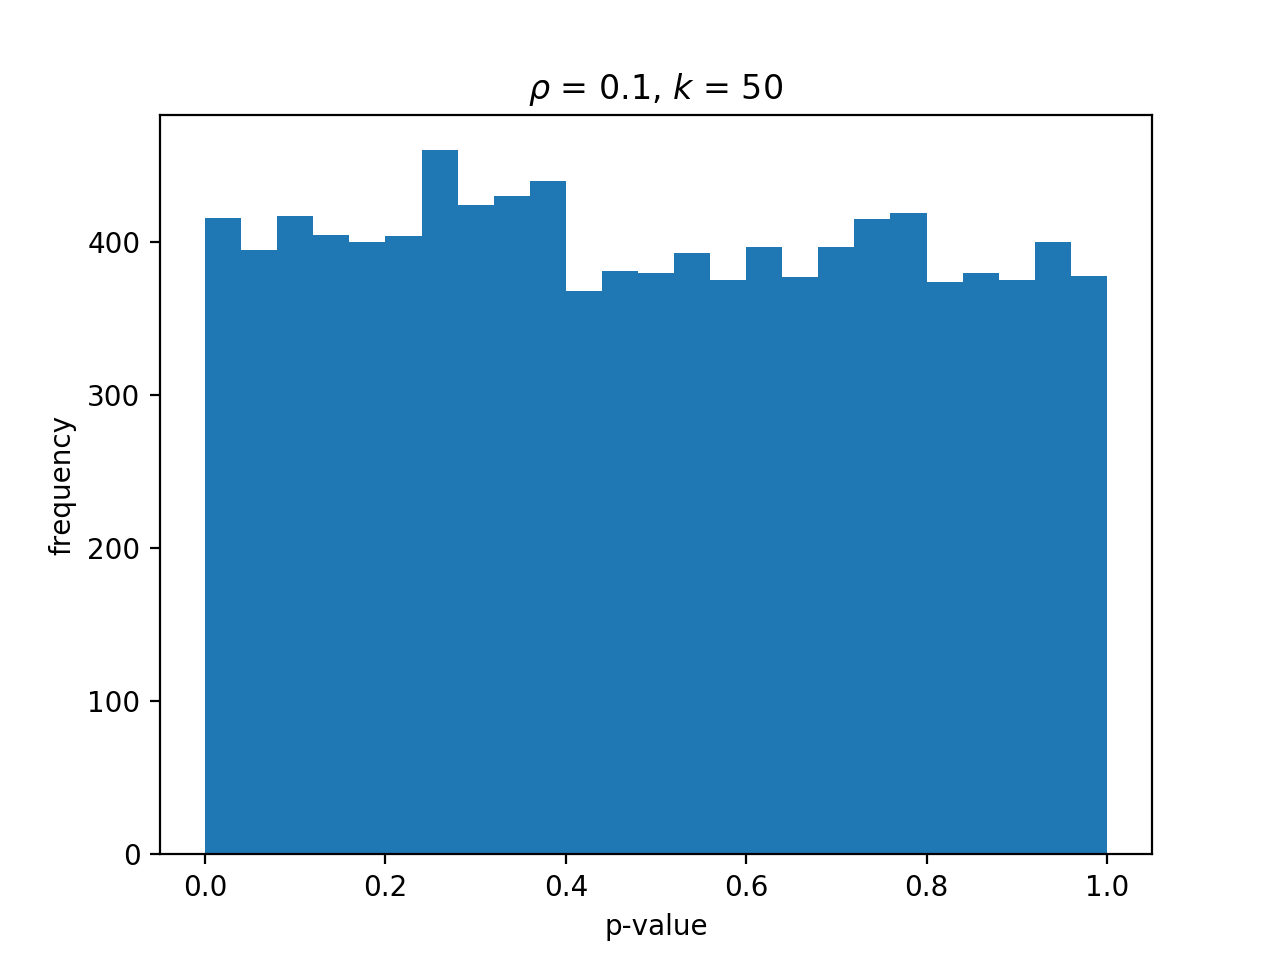
\includegraphics[width=0.33\linewidth]{rho01k50.png}
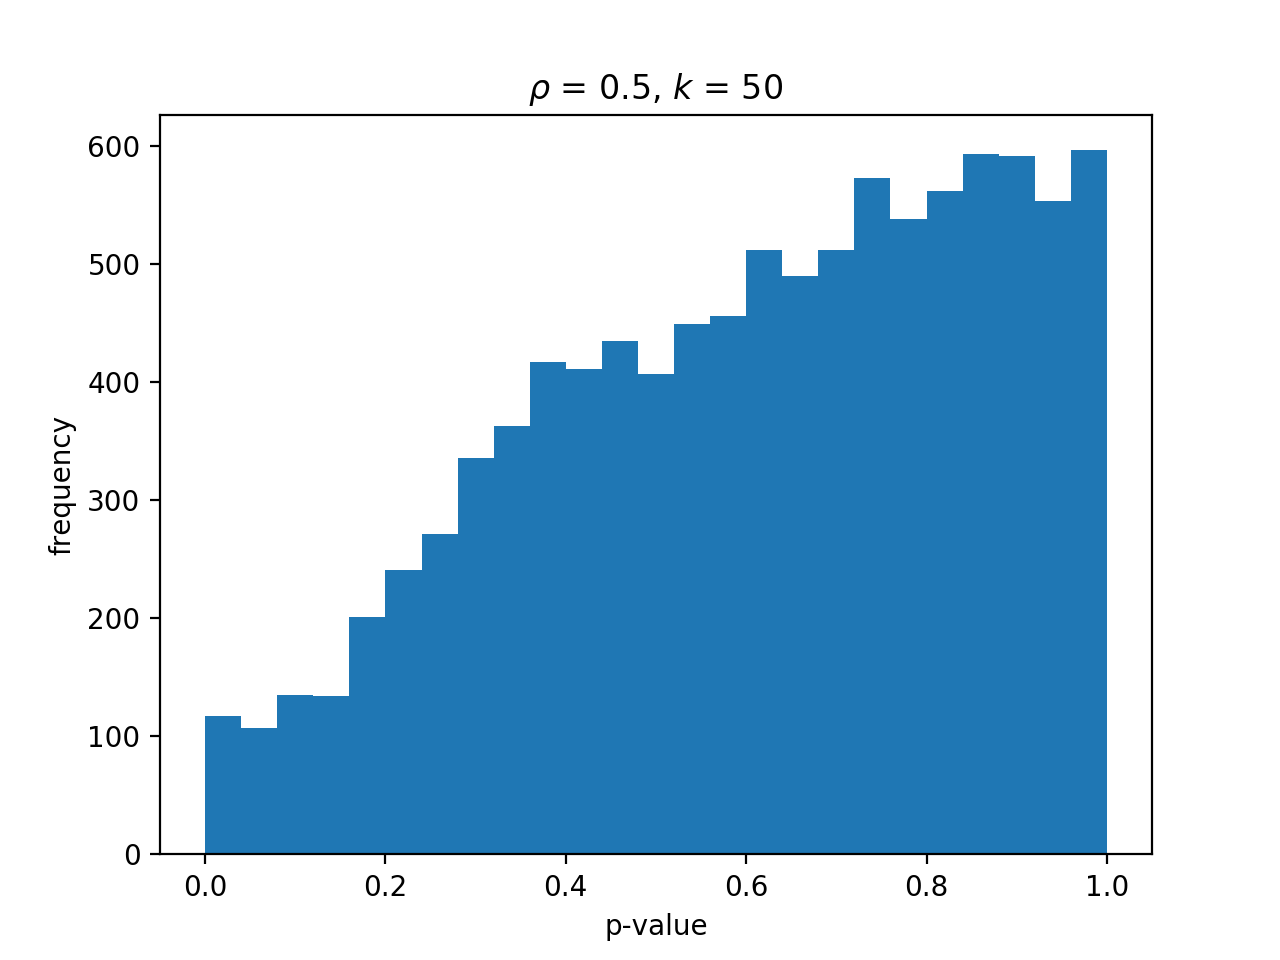
\includegraphics[width=0.33\linewidth]{rho05k50.png}
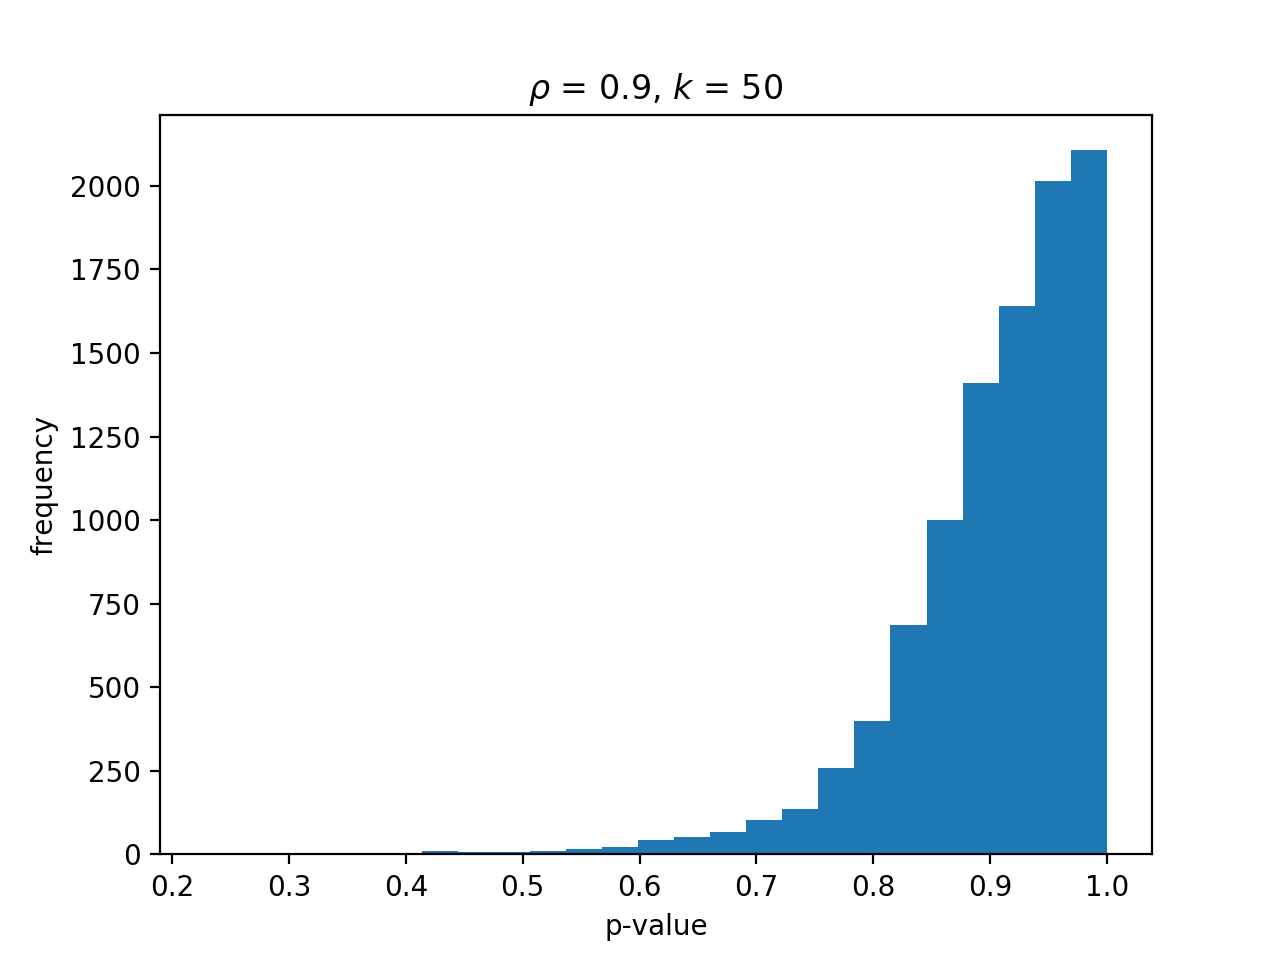
\includegraphics[width=0.33\linewidth]{rho09k50.png}

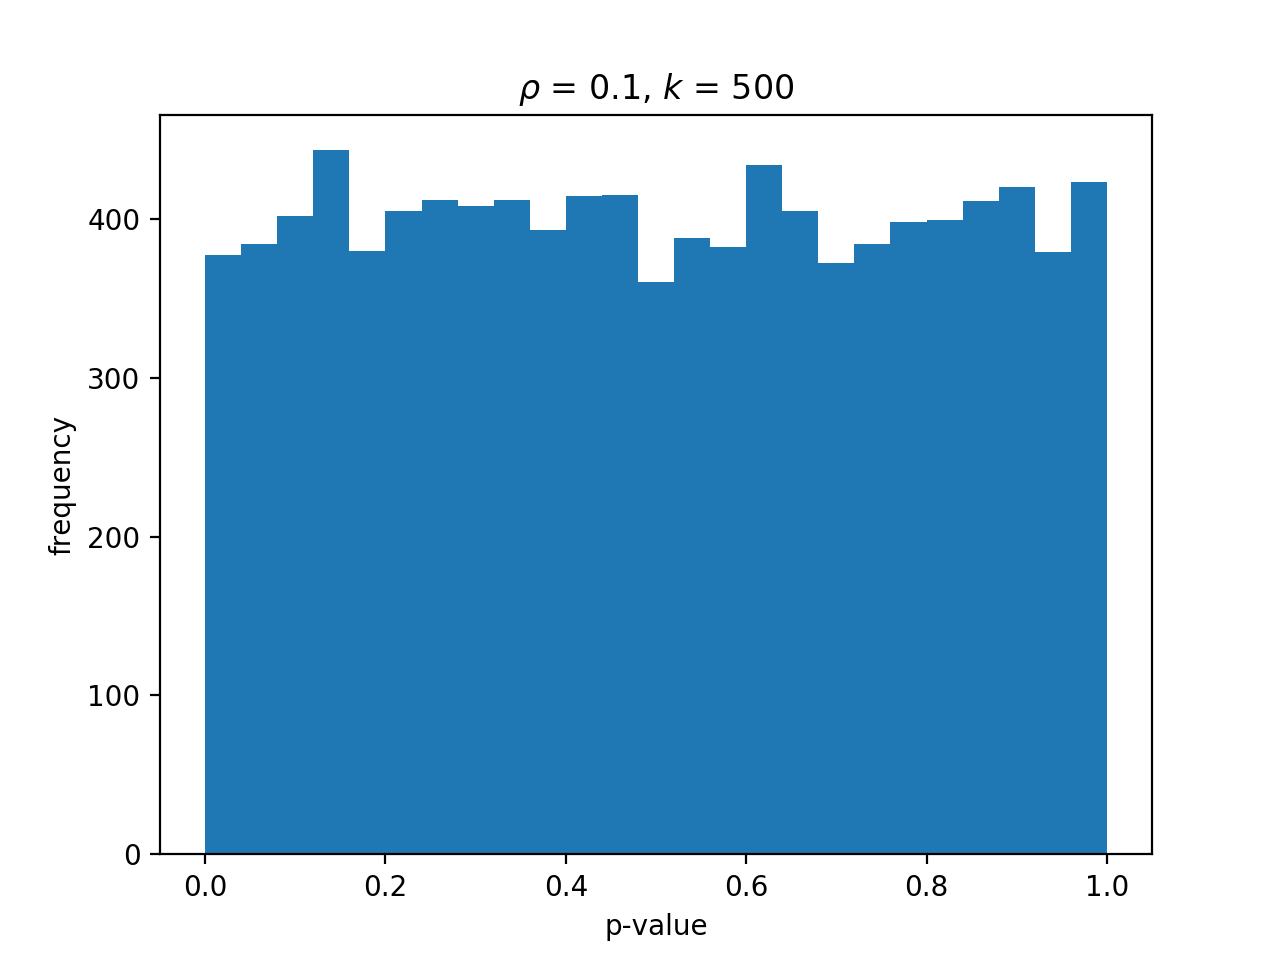
\includegraphics[width=0.33\linewidth]{rho1k500.png}
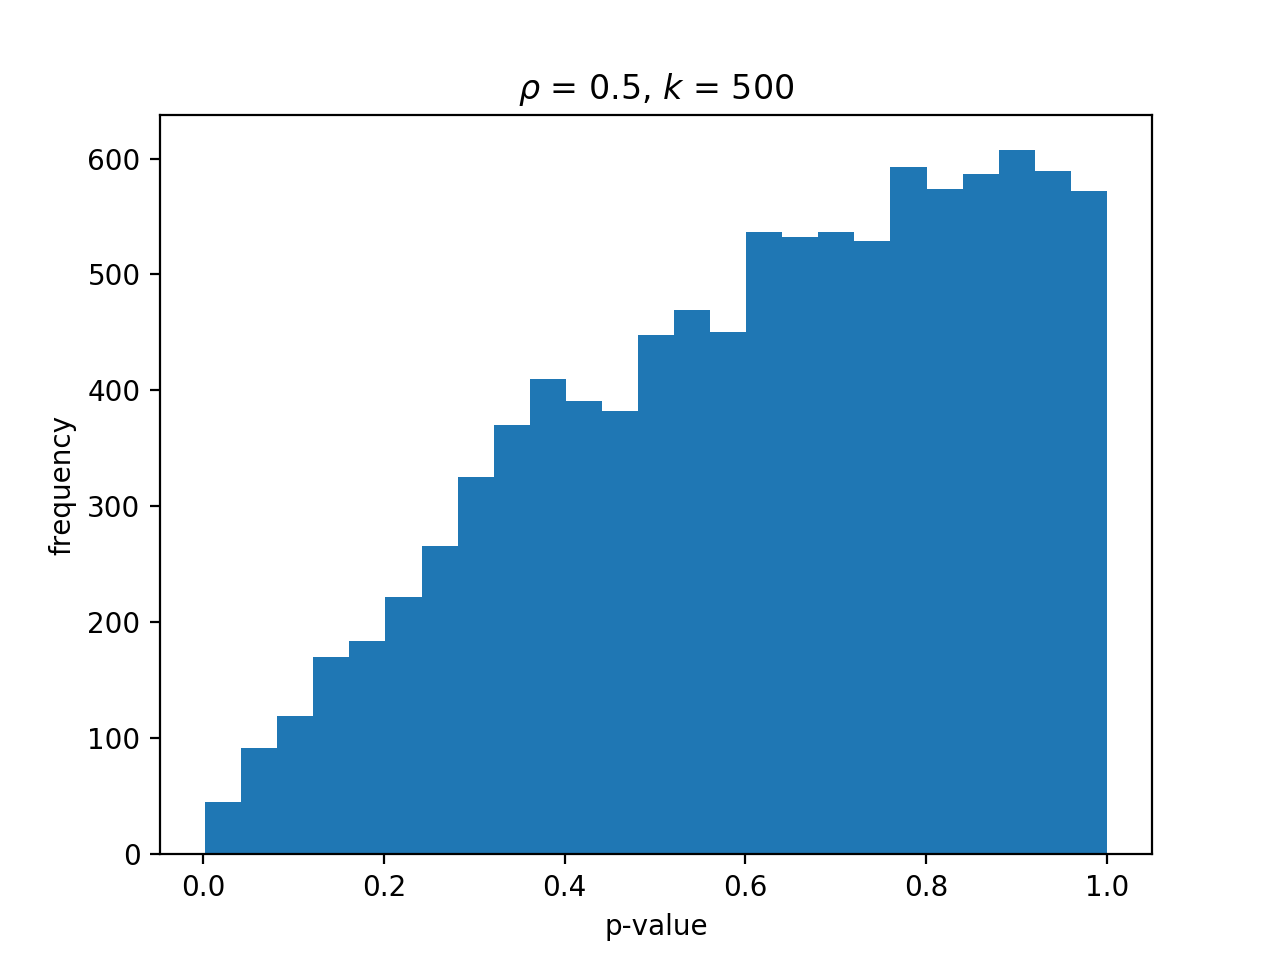
\includegraphics[width=0.33\linewidth]{rho05k500.png}
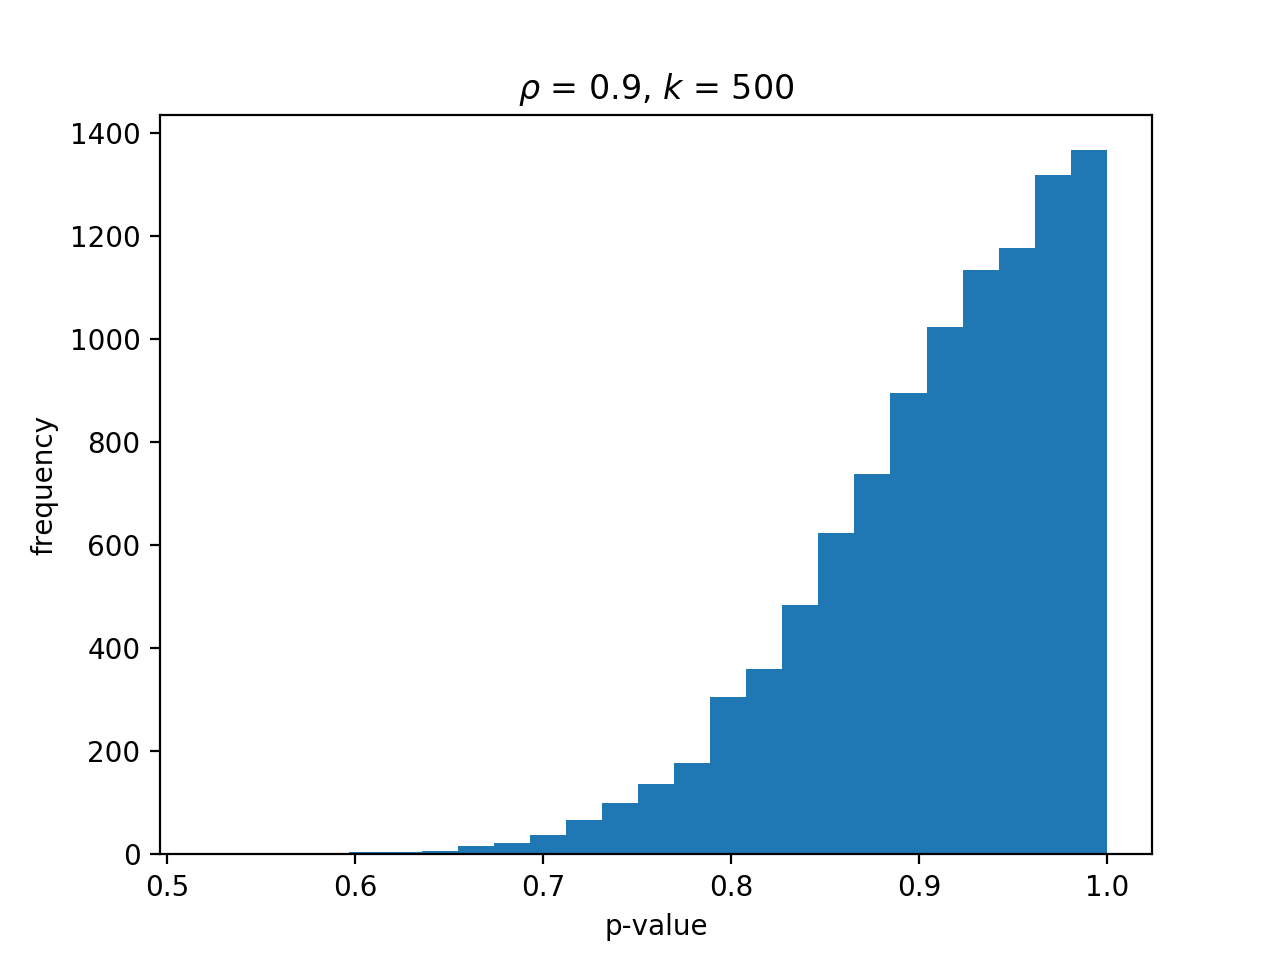
\includegraphics[width=0.33\linewidth]{rho09k500.png}

If the approximation worked well, we would expect that $p$-values would be uniformly distributed. We see that this is the case for $\rho = 0.1$. Unfortunately, for high $\rho$, we see that the approximation breaks down. We see that in cases where the two series are highly correlated that the chance of a low $p$-value is very low. However, while this isn't optimal, it also isn't terrible as it just means that the false-positive rate of detecting anomalies will be lower.

\section{Improvements}

There are several things that could be improved for our model.

\subsection{Detecting out-of-range failures}

Since our model is based on the shape of the data itself, it can detect subtle in-range failures but will not work well for out of range failures that do not otherwise have some anomalous shape.

\subsection{Changing how we compute $p$-values}

We can see from the graphs in the previous section that the test does not give a uniform distribution of $p$-values as we would hope. In his paper, "A note on the distribution of the product of zero mean correlated normal random variables", Gaunt describes a way that $r_i$ should be distributed if we assume $X$ and $Y$ are normal (this is another assumption, but it may be a better one than assuming $r_i$ is normal). We tried to implement this model initially, but gave up after running into issues with the numerical integration.

\end{document}






















